\chapter{Collaborative Navigation}
Collaborative Navigation (CN, also known as cooperative or
peer-to-peer navigation) is an approach where the navigating
units within the same area share their location and possibly
other information. CN is based on two central assumptions.
First, that each individual user is able to independently estimate their navigation state and state uncertainty, and second
that they have the ability to measure or estimate range and
range uncertainty to other cooperating users then communicate
the result to them. By exchanging in real time estimates of
state, relative range and state uncertainty each cooperating user
reduces the rate at which the error of the group of cooperating
users accumulates. In this, the authors are computing the
navigation solution for one user (target user U) by using
the visual odometry, IMU and barometer measurements and
then improving the solution by using collaborative navigation
via measuring range between the user and another user in
the group (initiating user S). The range is measured by
transmitting signals using Ultra-Wide Band (UWB) sensors
and computing the Round Trip Time (RTT) of transmitted and
received signal as shown in Figure 3.1 and (4).
\begin{center}
   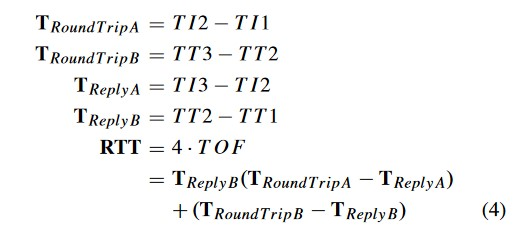
\includegraphics{eq4.jpg}
   \end{center}
\begin{figure}
    \centering
    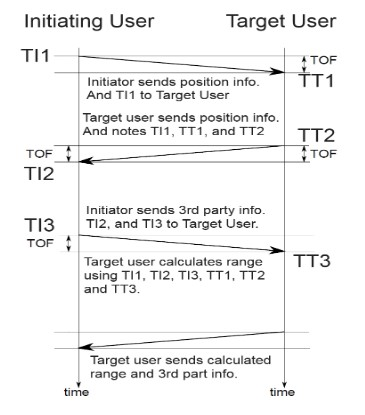
\includegraphics{fig8.jpg}
    \caption{Computing the Round Trip Time solution.}
    
\end{figure}   
In this study, an Extended Kalman filter (EKF) was used
for estimating the state vector xk including 16 states, namely
the position \begin{math}(x, y, z)\end{math}, velocity\begin{math} (v_x , v_y , v_z )\end{math}, attitude (pitch,
roll, yaw), gyroscope bias \begin{math}(g_x , g_y , g_z )\end{math}, accelerometer bias \begin{math}(a_x , a_y , a_z )\end{math} and barometer bias \begin{math}(b_z )\end{math}. The state is predicted
using the visual odometry, IMU, and barometer measurements.
As is implicit in the state selection, integration of aiding
sensors with the IMU is accomplished via ‘loose’ coupling,
typically via the position and or velocity states depending on
the specific source. The noise model adopted assumes white
gaussian noise dominates from the INS accelerometers and
gyroscopes, while the accelerometer and gyroscope bias states
are modelled as first order Markov processes.\\
The measurement model relating the RTT measurements
with the state is  
\begin{center}
   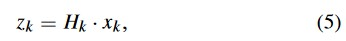
\includegraphics{eq5.jpg}
   \end{center}
where \begin{math}H_k = [dxdp, dydp, dzdp, 0, . . ., 0]\end{math}. The \begin{math}dxdp\end{math} term
is calculated from the predicted position X-coordinate of the
initiating user (S) and target user (U) as   
\begin{center}
   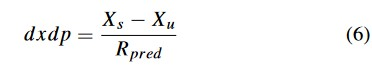
\includegraphics{eq6.jpg}
   \end{center}
and \begin{math}R_p_r_e_d\end{math} is   
\begin{center}
   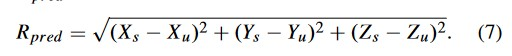
\includegraphics{eq7.jpg}
   \end{center} 
\begin{math}dydp\end{math} and \begin{math}dzdp\end{math} are computed similarly using the predicted Y
and Z coordinates, respectively.\\
Additional performance is achieved through sharing of
specific state flags which reflect whether for example a user
is presently static (ZUPT condition) or whether a user has an
independent ability to measure its position such as a GNSS
fix. These conditions frequently arise when some but not
all members of a team enter a building, denying GNSS to
those inside but often still allowing the higher power RTT
and communications signals to pass through the building.
In this study, decentralized collaborative navigation was
pursued in order to allow the cooperating group of users
to dynamically fragment and reform without disruption as
communication through building material allowed at any given
time. While the benefit of decentralized processing is the
implicit tolerance of the ensemble to communication dropouts,
a primary drawback is the need to mitigate the impact of the
circulation of ‘stale’ data which in this study was addressed
through injection of stabilizing noise to the position state of
users operating without an external reference. In order to
reduce the impact of information re-circulation within the
network, an additional noise term is added to the position
states of the Q matrix of each user with density equivalent
to a 5 metre uncertainty in each axis after 5 minutes of
operation, but is only applied to dynamic users without GNSS
reference. Users under ZUPT conditions or with an external
position solution do not receive this Q matrix modification.
Situational awareness is maintained through the forwarding
of 3rd party state information such that even a single point
of contact shared between two groups of users will allow
knowledge of the others state even if range measurement
between two given users is at that point not possible due to
building material obstruction. Since the measurement model
makes direct use of the estimated position states of both the
initiating and responding user, the formed vector is both scaled
and rotated by position state errors in either user. For constant   position uncertainty in the initiating and target users, the error
in the direction of the vector formed in equation 6 will tend to
grow larger with decreasing predicted range. To account for
this, the measurement covariance matrix for inter-user ranging
measurements is de-weighted when Rpred values fall below
5 metres.